\startchapter{Language Idioms}
\label{chapter:idioms}

\section{Introduction}
In this chapter, We begin by explaining our approach to \textbf{RQ-1.1} (How do \cct{} manage programming idioms?). To achieve this, we conduct an exploratory study to find if \cct{} tools like Copilot suggest the optimal way in their suggestions. It is shown that Copilot's base model Codex performs best in python programming language~\cite{copilot}. So, we chose to test Copilot on python programming language idioms.

In section~\ref{methodology}, we describe our sampling approach to collecting python idioms and evaluation method used to compare copilot suggestions to the optimal way listed in python idioms. In section~\ref{secidioms}, we show the results of the study comparing Copilot suggestions and idioms in python programming language. We observe that Copilot performs poorly in suggesting the optimal way in its suggestions. 
\section{Pythonic Idioms}
The definition for the term \emph{Pythonic} in Python found in official Python glossary\footnote{\url{https://docs.python.org/3/glossary.html\#term-pythonic}} as follows:

\begin{quote}
    An idea or piece of code which closely follows the most common idioms of the Python language, rather than implementing code using concepts common to other languages. For example, a common idiom in Python is to loop over all elements of an iterable using a for statement. Many other languages do not have this type of construct, so people unfamiliar with Python sometimes use a numerical counter instead, as opposed to the cleaner, pythonic method.
\end{quote}

This definition indicates a broad meaning, referring to both concrete code, but also \emph{Ideas} in general sense. Many Python developers argue that coding the \emph{pythonic way} is the most accepted way to code by the Python community~\cite{Alexandru2018}. We consider an \emph{idiom} to be any reusable abstraction that makes Python code more readable by shortening or added syntactic sugar. Idioms can also be more efficient than a basic solution and some idioms are both more readable and more efficient.

We sampled idioms from the work of Alexandru et al.~\cite{Alexandru2018}, which identified idioms from presentations given by renowned Python developers that frequently mention Idioms, e.g., Hettinger~\cite{hettinger} and Jeff Knupp~\cite{knupp} and popular Python books, such as ``Pro Python''~\cite{Alchin2010}, ``Fluent Python''~\cite{fluent}, ``Expert Python Programming''~\cite{expert}.

\section{Methodology}
\label{methodology}
In this Section, We explain the methodology we used to address \textbf{RQ-1.1} (How do \cct{} manage programming idioms?), including how the idioms were sampled (Section~\ref{sampling}), what was the input for Copilot (Section~\ref{input}) and how Copilot suggestions are evaluated (Section~\ref{evaluation}). All of the following analysis was carried out using Copilot extension in Visual Studio Code. We use the most recent stable release of Copilot extension (version number 1.30.6165) in Visual Studio Code.

\subsection{Sampling Approach}
\label{sampling}
To give the best chance for Copilot to suggest the optimal way, we sampled the top ten most frequent idioms used in open source projects. So that, Copilot will have the optimal way more frequently in its training data. However, Copilot is closed source and we cannot determine if the frequency of code snippet in training data affects Copilot suggestions in any way. Research by GitHub shows that Copilot can sometimes recite from its training data in ``generic contexts"\footnote{\url{https://github.blog/2021-06-30-github-copilot-research-recitation/}}, which may lead to potential challenges like licence infringements~(shown in section~\ref{challenges}). Sampling the most frequently used idioms will also help understand if Copilot can recite idioms present in its training data~(GitHub public repositories), which is a desirable feature for \cct{}.

\subsection{Study Setup}

\subsubsection{Input to Copilot}
\label{input}
The input to Copilot consisted of the idiom title in the first line as a comment to provide context, and the input was restricted to being able to derive the ideal way~(idiomatic way) from the input. This is done to ensure Copilot is making the decision to suggest the good/bad way in its suggestions and not being restricted by the input to suggest a certain way. 

This input style also mimics a novice user, who is unaware of the idioms and useful \cct{} should drive the novice user to use idiomatic ways to perform a task in their codebases.

\subsubsection{Evaluation of Copilot suggestions}
\label{evaluation}
We considered Copilot suggested the optimal way if Copilot suggested the idiomatic way in the first suggestion, we assume that \cct{} like Copilot are productivity tools and user should be saving time as opposed to writing the optimal way without using \cct{}, scrolling through all the suggestions to deduce the optimal way defeats this purpose. For this reason, we restricted ourselves to first suggestion. However, we do note if the idiomatic way appeared any of the top 10 suggestions currently viewable in Copilot interface. 

% including sections in other files.
\section{Results}
\label{secidioms}
Using the methodology described in section~\ref{methodology}, we picked the top 10 most popular python idioms from work of Alexandru et al.~\cite{Alexandru2018} and compared Copilot suggestions when prompted with a input method~(shown in section~\ref{input}) and evaluated using methodology shown in section~\ref{evaluation}. 

Copilot suggested the idiomatic approach as the first suggestion in 2 of the 10 idioms we tested i.e., 2 out of 10 instances Copilot had the recommended way as its top suggestion. However, 4 out of those remaining 8 Idioms had the idiomatic way in Copilot's top 10 suggestions. Copilot did not have the idiomatic way in any of its top 10 suggestions for 4 idioms out of 10 idioms we tested.

Table~\ref{tab:all_idioms} shows the list of all the 10 idioms we tested and the ranking of the idiomatic way in Copilot suggestions (if it exists).

\renewcommand{\arraystretch}{1.7}
\begin{table}[ht]
    \centering
    \begin{tabular}{|L|c|}
    \hline
         \textbf{Idiom Title} & \textbf{Copilot Suggestion Matched?} \\
         & (out of 10 suggestions) \\
         \hline
         List comprehension & No \\
         \hline
         Dictionary comprehension & No \\
         \hline
         Mapping & 9\textsuperscript{th} \\
         \hline
         Filter &  7\textsuperscript{th} \\
         \hline
         Reduce & 9\textsuperscript{th} \\
         \hline
         List enumeration & No \\
         \hline
         Set comprehension & 1\textsuperscript{th} \\
         \hline
         Read and print from a file & 5\textsuperscript{th} \\
         \hline
         Add int to all list numbers & No \\
         \hline
         If condition check value & 1\textsuperscript{th} \\
         \hline
    \end{tabular}
    \caption{List of all python idioms tested on Copilot.}
    \label{tab:all_idioms}
\end{table}


Figure~\ref{fig:idioms_1} shows the example of list comprehension idiom, showing user input (i.e., human input), the top suggestion by Copilot and the idiomatic way from Alexandru et al.~\cite{Alexandru2018}.

\begin{figure}[hbt!]
    \centering
    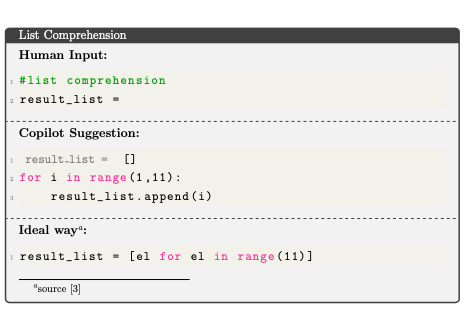
\includegraphics[width=\linewidth]{Figures/idioms_1.png}
    \caption{List Comprehension Idiom and Copilot Suggestion}
    \label{fig:idioms_1}
\end{figure}

The results show that Copilot did not suggest the optimal way as its first suggestion in the majority of the idioms we tested. This shows that current \cct{} like Copilot cannot suggest the idiomatic way in every suggestion even though they are the top most frequently used python idioms in public repositories on GitHub~\cite{Alexandru2018}. 

Copilot being closed source we cannot investigate the potential reasons behind this behavior. However, one plausible explanation for this behavior is that idiomatic ways may not be as frequent as non-idiomatic ways in Copilot's training data of public repositories on GitHub, making the non-idiomatic way rank higher than the idiomatic way.

\cct{} like Copilot should learn to detect idiomatic ways in public repositories and rank them higher than the most frequently used way in public repositories, so that the first suggestion would be the idiomatic way rather than the non-idiomatic way, which is the desirable way for \cct{} like Copilot. For the scope of this thesis, we leave resolving this problem as future work.

% \begin{tcolorbox}[title=List Comprehension,boxsep=.25mm]
%     %https://tex.stackexchange.com/questions/337909/tcolorbox-tcbline-style
% \textbf{Human Input:}
% \begin{lstlisting}[language={Python}]
% #list comprehension
% result_list = 
% \end{lstlisting}
% \tcbline
% \textbf{Copilot Suggestion:}
% \begin{lstlisting}[language=Python,escapechar=\%]
% % \noindent\textcolor{gray}{result\_list  =} % []
% for i in range(1,11):
%     result_list.append(i)
% \end{lstlisting}
% \tcbline
% \textbf{Idiomatic way\footnote{source \cite{Alexandru2018}}:}
% \begin{lstlisting}[language=Python]
% result_list = [el for el in range(11)]
% \end{lstlisting}
% \end{tcolorbox}

%%%%%% TODO: remember to update the screenshot if the source citation is different from the citation in the text %%%%%%

All the Idioms shown in Table~\ref{tab:all_idioms} can be found in the \repl{} including the code used as input (i.e., human input), the top suggestion by Copilot and the idiomatic way suggested in Alexandru et al.~\cite{Alexandru2018}.

\section{Chapter Summary}
In summary, we start this chapter by showing the methodology used in addressing textbf{RQ-1} (What are the current boundaries of \cct{}?). 
We first introduced Pythonic idioms and best practices in JavaScript.
We then present our sampling approach for sampling 25 coding scenarios to analyze Copilot code suggestions.
Furthermore, we discussed the input given to Copilot to trigger a code suggestion 
and how the input was restricted to deriving the desired way from the input.
Finally, we described our evaluation approach for Copilot code suggestions.

We sampled 25 Pythonic idioms from Alexandru et al.~\cite{Alexandru2018}, and Farook et al.~\cite{idioms}.
We identified that Copilot did not suggest the idiomatic way as its top suggestion for 23 out of 25 coding scenarios in Python, which addressed \textbf{RQ-1.1} (How do \cct{} manage programming idioms?).
Furthermore, we sampled 25 best practices in JavaScript from the AirBNB JavaScript coding style guide~\cite{airbnb_code}. We identified that Copilot did not suggest the recommended best practice for 22 out of 25 coding scenarios in JavaScript, which addressed \textbf{RQ-1.2} (How do \cct{} manage to manage to suggest non-smelly code?).


% we showed that Copilot struggles to detect and most common idiomatic ways present in public repositories of GitHub and rank them higher than the non-idiomatic ways. The ideal behavior of \cct{} like Copilot in solving this problem is detecting common patterns present in code and rank them higher as the idiomatic ways for a task.
% In the next chapter (chapter~\ref{smells}), we look into how this ideal behavior can cause problems in the case of code smells, where common bad practices present in public repositories of GitHub can make \cct{} like Copilot introduce bad coding practices in its suggestions.

% % \section{Chapter Summary}
% In summary, we start this chapter by showing the methodology used in addressing \textbf{RQ-1.2} (How do \cct{} manage to suggest non-smelly code?). We first introduced the study setup with the input to Copilot and how it was restricted to deriving the best practice from the input and how the suggestions from Copilot were evaluated. We sampled best practices from AirBNB JavaScript coding style guide~\cite{airbnb_code}, and then compared it against Copilot suggestions. Based on results shown in Table~\ref{tab:all_bp}, Copilot struggles to suggest the best practices from widely used coding standards in its suggestions. 

In this chapter, we showed that Copilot struggles to detect and follow coding style guides present in public repositories of GitHub and always suggests code that follows those coding style guides. We also observed that Copilot struggles to detect and most common idiomatic ways present in public repositories of GitHub and rank them higher than the non-idiomatic ways. 
Identifying this delineation could help in urn AI-supported code completion tools such as Copilot into full-fledged AI-supported software engineering tools.
In the next chapter (chapter~\ref{chapter:framework}), we illustrate our taxonomy inspired by autonomous driving levels on the software abstraction hierarchy in \AISE{} and delineate where \cct{} like Copilot currently stands in the taxonomy. 